\documentclass{article}%
\usepackage[T1]{fontenc}%
\usepackage[utf8]{inputenc}%
\usepackage{lmodern}%
\usepackage{textcomp}%
\usepackage{lastpage}%
\usepackage{authblk}%
\usepackage{graphicx}%
%
\title{Anti{-}inflammatory effect of aldose reductase inhibition in murine polymicrobial sepsis}%
\author{Rhonda Knight}%
\affil{Instituto de Biologa Molecular y Celular de Plantas, Universidad Politcnica de Valencia{-}C.S.I.C, Ciudad Politcnica de la Innovacin, Valencia, Spain}%
\date{01{-}01{-}2013}%
%
\begin{document}%
\normalsize%
\maketitle%
\section{Abstract}%
\label{sec:Abstract}%
SURPRISE, Ariz.  A team of researchers at UCSF has created a new genetically modified mouse model that can successfully produce one of the most successful stem cell lines in breast cancer  in a brain cancer patient.\newline%
The decedent had been undergoing chemotherapy when she had tumors in her brain stem and a small tumor on the lower back. Instead of facing death, she was spared further treatment due to the therapy. The tumor had spread and the disease also spread to her lymph nodes.\newline%
The researchers hope to pinpoint the mutated cells and use them to help develop new drugs to block metastases, and stem cell transplantation for patients whose tumors are directly related to the diseases.\newline%
This type of cancer kills about 50,000 women a year in the United States, according to the American Cancer Society.\newline%
Its like hunting for new ways to prevent cancer in individuals so the only thing we have left is to keep finding new cures, said lead researcher Dr. Abigail Chincote, a senior research scientist at UCSF and one of three UCSF researchers whose work contributed to the paper that appeared in the Proceedings of the National Academy of Sciences (PNAS).\newline%
The researchers from UCSF, Japan, and the University of Michigan also collaborated with researchers at the U.S. Food and Drug Administration and Chinese health officials in Beijing, Changsha, Kolkata, Bangalore, and Hong Kong to grow the mouse model at a laboratory controlled by the Chinese government.\newline%
In the study, they utilized a new genetic modification to create an embryo of a tumor cell directly removed from the tumor before being placed in a culture medium containing normal cells. The cells had genetic modifications allowing the embryo to grow as well as to multiply and to generate the most capable stem cells.\newline%
The first cells that grew produced tens of thousands of tumor cells.\newline%
Stem cells are just like kids playing with their toys. They react to things, but some of the cell types in human breast cancer are much more resistant to these modifications, Chincote said.\newline%
The cell mutations were found in those tumors that presented tumors such as the BRCA1 and BRCA2 gene mutations, but all mice grown outside the body were unaffected.\newline%
The researchers next tested the engineered mouse model to find out if it could be administered either to patients diagnosed with a breast cancer{-}associated tumor in the head or a GBL chemotherapy{-}induced metastasis on the back.\newline%
The trial revealed that the engineered mice that were given chemotherapy{-}induced metastasis had much less tumor growth in the brain than the tumors that originated on the bone and in the spinal cord that the cancerous cells were able to spread to.\newline%
The median survival rate was 71 percent for the mice who received chemotherapy{-}induced metastasis. Another study found that the healthy mice that were injected with a substance called opsin using ductal carcinoma extracellular matrix (DCM) can endure chemotherapy to only a third of the strength of the chemotherapy dose placed on them before the cancerous cells were discovered.\newline%
Chincote also called the mouse models critical to future strategies for fighting the disease in humans.\newline%
We want to see if the development of these mouse models can be able to produce tumors that grow in person, but many of the cancer cells can disappear, she said.

%
\subsection{Image Analysis}%
\label{subsec:ImageAnalysis}%


\begin{figure}[h!]%
\centering%
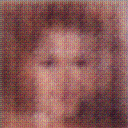
\includegraphics[width=150px]{500_fake_images/samples_5_294.png}%
\caption{A Man In A Suit And Tie In A Room}%
\end{figure}

%
\end{document}